\documentclass{sig-alternate}
\usepackage[utf8]{inputenc}
\usepackage{times}
\usepackage{gensymb}
\usepackage{epsfig}
\usepackage{xcolor}
\usepackage{xspace}
\usepackage{multicol}
\usepackage{listings}
\usepackage{verbatim}

\begin{document}
\conferenceinfo{CIDR '17}{January 8-11, 2017, Santa Cruz, CA, USA}
\newcommand{\smallitem}[1]{\vspace{1em}\noindent\textbf{#1}}
\newcommand{\smallitembot}{\vspace{1em}\noindent}
\bibliographystyle{abbrv}

\newcommand{\jmh}[1]{{\textcolor{red}{[[#1 -- jmh]]}}}
\newcommand{\joey}[1]{{\textcolor{cyan}{[[#1 -- jeg]]}}}
\newcommand{\msd}[1]{{\textcolor{green}{[[#1 -- msd]]}}}
\newcommand{\akon}[1]{{\textcolor{orange}{[[#1 -- akon]]}}}

\newcommand{\vikram}[1]{{\textcolor{blue}{[[#1 --vikram]]}}}
% \newcommand{\jmh}[1]{}

\newcommand{\vml}{VML\xspace}
\newcommand{\core}{bedrock\xspace}
\newcommand{\mantle}{central\xspace}
\newcommand{\crust}{top\xspace}
\newcommand{\Core}{Bedrock\xspace}
\newcommand{\Mantle}{Central\xspace}
\newcommand{\Crust}{Top\xspace}

\newcommand{\version}{\texttt{Version}\xspace}
\newcommand{\richversion}{\texttt{RichVersion}\xspace}
\newcommand{\thing}{\texttt{Thing}\xspace}
\newcommand{\node}{\texttt{Node}\xspace}
\newcommand{\edge}{\texttt{Edge}\xspace}
\newcommand{\structure}{\texttt{Structure}\xspace}
\newcommand{\graph}{\texttt{Graph}\xspace}
\newcommand{\TVID}{\texttt{TVID}\xspace}
\newcommand{\gtag}{\texttt{Tag}\xspace}
\newcommand{\uri}{\texttt{URI}\xspace}

\newcommand{\versiongraph}{version graph\xspace}
\newcommand{\modelgraph}{model graph\xspace}
\newcommand{\lineagegraph}{lineage graph\xspace}
\newcommand{\versiongraphs}{version graphs\xspace}
\newcommand{\modelgraphs}{model graphs\xspace}
\newcommand{\lineagegraphs}{lineage graphs\xspace}
\newcommand{\groundwire}{GroundWire\xspace}


\title{Grounding Big Data with Data Context Services}
\numberofauthors{3}
\author{
Groundlings
}

\maketitle

\begin{abstract}
Ground is an open-source data context service, motivated by our experiences in the Big Data ecosystem. By data context, we refer to all the peripheral information that informs the use of data, going well beyond traditional metadata.
The way we use data has changed both philosophically and practically in the last decade, creating an opportunity for new data context services to foster further innovation in Big Data systems and applications. We provide motivation and design guidelines, present our initial design of a common metamodel and API, and explore the current state of the storage solutions that could serve the needs of a data context service. Throughout, we highlight opportunities for new research and engineering solutions.
\end{abstract}

\section{From Metadata to Context}
The open-source Big Data movement, spearheaded by Apache Hadoop, is often discussed in terms of changes in usage: the ``three V's'' \msd{perhaps spell out the three Vs here} of the data being captured and the agile working style typified by ``schema-on-use'' and polyglot programming models.

Much less widely discussed is a profound shift toward a decoupled software architecture. Traditionally, database systems were consumed as monolithic stacks of component functionality, regardless of how well-factored they were under the covers. \msd{Although} A DBMS included a consistent storage engine, a metadata catalog, a dataflow engine, a language compiler and optimizer, an execution scheduler/runtime, and facilities for data ingest and queueing \msd{, it was simply seen as a DBMS}. In today's Big Data stack, nearly all of these components are \msd{explicitly} independent and swappable. Moreover, there are multiple choices for most of these components in wide use today. The decoupled architecture is healthy for innovation and specialization, and has been embraced by both developers and customers.

One negative side-effect of this diversity is the lack of an agreed-upon service to register metadata \msd{metadata or data context?} for these components. The only widely-used solution is the Hive Metastore, which serves simple relational schemas---a dead end for Variety. As a result, most ``Data Lake'' projects lack even the most basic information; typically it is not even possible to discover what is being stored. 
For emerging Big Data customers and vendors, this Big Metadata problem is hitting a crisis point.  Two serious problems emerge.

\jmh{Funny transition from software stack problem to usage problem. Need to start with interoperability and grow from there, or change preceding paragraph to focus on usage not the stack.}
\joey{What are the problems? Could we introduce the ``Vs'' of meta-data management: Discovery, Provenance, Attribution, Context ..., if we could articulate these clearly then we could perhaps translate their implications on administration, loss-of-value, risk to organization, ... }
The first is poor productivity.
%The promise of the Data Lake is that a diversity of data can be easily captured, and then harnessed by analysts for value. 
In the absence of metadata, analysts are often unable to discover what data exists, much less how it may have been previously parsed, structured, cleansed and analyzed by peers. ``Tribal knowledge'' in an organization is the standard method for disseminating this information today. Clearly this does not scale, leading to wasted work and lost opportunities for analysts to build on the data and analysis known to others.

The second problem is governance risk. Data management necessarily entails recording governance information: who accesses data, what they do with it, where they put it, and how it gets consumed downstream. 
%In some cases this governance metadata is used to enforce policy (e.g.\ access control for Personally Identifiable Information); in others it is logged to support audits for compliance (e.g.\ in the Basel Committee on Banking Supervision). 
In the absence of a standard place to store and access this information, it is impossible to enforce policies and/or audit behavior. As a result, many administrators marginalize their Big Data stack as a playpen for non-sensitive data.\msd{and thereby inhibit both the adoption and the potential of Big Data technologies.}

In our diverse experiences in industry, the authors have seen a pressing need for a common service layer to let Big Data components ``write down'' and share metadata information in a flexible way \msd{perhaps "document, publish, and share data context"}. The effort in this paper began by addressing that need.

\subsection{Opportunity: The ABCs of Context}
The lack of metadata services in the Big Data stack is not just a crisis; it is also a clean-slate opportunity to rethink design and usage. Storage economics and the simplicity of schema-on-use suggest that the Data Lake movement could go much farther than Data Warehouses in enabling diverse, widely-used central repositories of data.

In that spirit, we advocate rethinking traditional metadata in a far more comprehensive sense, expanding focus to the full \emph{context} that informs data and its usage. To accompany the three V's of Big Data, we introduce the \emph{ABCs of Data Context}:

\msd{not sure where some of these metadata items would fit in: (1) business metadata (keywords, classification, compliance details, end-user tags), (2) operational metadata (date and execution details), (3) etc. - perhaps a bullet point list of the types of metadata and how it fits into ABC categories might help. I'm not sure that ABC covers the full scope.
}\jmh{Took a crack at making sure these could fit in. See discussion after the list about whether to be explicit here.}

\jmh{Want to make sure that we get each of A, B and C to have simple stories about what's novel. Right now it's in notes; ideally we find a paragraph structure where it fits into each paragraph neatly. Or we could have a separate table...}

\smallitem{A: Application Context}: This is the core information that describes how raw data (e.g. bits on disks) gets interpreted for use. It includes basic data descriptions (schemas, ontologies, tags), statistical models and parameters, end-user annotations, etc.  Application context is often bespoke, specific to a single use case or set of use cases. But some application context is intended to be universally applied across applications; e.g., access control or privacy information. Note that the interpretation of raw data typically requires executing code. Hence the artifacts involved in that code---the transformation scripts, view definitions, model parameters, training sets, etc.---all become critical parts of recreating application context. \jmh{Novelties: subjectivity of models, inclusion of richer detail including code.}
% Application context includes both metadata and code.

\smallitem{B: Behavioral Context}: This is information about how data was created and used over time. It includes the upstream lineage of a particular data object: the data sets and code that led to the creation of the object. It includes any downstream lineage as well: data products that were derived from this data object. In the new decoupled stack, this lineage comes from a diverse set of applications, languages and compute frameworks that access the data; it is likely to vary in granularity and interpretability.
Additionally, behavioral context includes logs of non-lineage producing usage of the object as well: the ``digital exhaust'' left behind by computations that touched the object, which can be used to predict future usage. Behavioral context can grow to be extremely large: often larger than the data itself. \jmh{Novelties: diverse forms of lineage, high-volume log data,}

\smallitem{C: Change Context}: This is information about the version history of data objects over time, including both the structure and content of the objects. It can be a linear sequence of versions, or it can encompass branching and concurrent evolution of objects across alternate versions, followed optionally by subsequent merges. Version history is familiar in the world of code, but here we want to track it for all kinds of data objects: code, atomic data items, and collections of data as well. \jmh{Novelties: versioning across both code and data, including singletons and collections.}
% If we view metadata more broadly, could a unified solution address a much broader set of goals than Data Warehouses? We can explore that notion along three axes:

% \smallitem{Data.} A schema-on-use world is inherently relativistic. Data does not have \emph{inherent} structure and meaning; rather, the structure is imposed post hoc---sometimes for general usage, sometimes for a specific task.  This means that the ``description'' of a collection of data depends not only on its original form, but on the (many) ways it is transformed for use over time.  

% \smallitem{Code}. Data is transformed by code, which becomes a necessary aspect of data description. Transformation is only one kind of data-centric code. There is also code that produces new data: analysis routines, statistical models, and outbound services like recommenders and ad systems. Data \emph{lineage} is a natural byproduct of code, relating it to data sources and outputs. Code also brings along data of its own: training data, model parameters, configuration files, etc. This is not the data of record in an organization; it is an aspect of the code itself. Code management brings its own requirements, notably information on versions, authors and testing.  
% %With code and data versioned over time we can envision robust reproducibility of experiments---a feature of interest in areas including hypothesis testing (e.g. A/B tests) and in scientific verification.  

% \smallitem{Usage}. In modern agile analytic environments, iterations of exploration, experimentation and (re)deployment of automated pipelines are daily activity. Ironically, today's Big Data software is not well-designed for enabling analysis of its own use. If people learn by doing, then the tribal knowledge of an analytic organization should be visible in its usage logs. Intelligent analytic software could take great advantage of these logs to augment and accelerate human activity and intelligence. Like all software usage logs, analytics logs are themselves big, diverse data.

\smallitembot
\jmh{Having written the below, I'm not sure this is a good idea to discuss here. My concern here is that in neatly covering all the old stuff we're diminishing the contrast. The Three V's are a mnemonic for ``what's different''---even if you don't really believe them!  Maybe this should go in Related Work. It should also be looked over by an ex-Informatica or ex-WebSphere person.}
\msd{I've re-read this section numerous times and feel that it doesn't fully capture the extent of motivation for this work that you've discussed very clearly in your live presentations. Perhaps this is best displayed as a graphic that shows the limited set of problems solved by the legacy approach to metadata juxtaposed with the expanded set of problems that can be solved by by data context; i.e., more clearly emphasize the delta (compliance: tracking access holistically, capturing data movement holistically, maintaining traceability of calculations; productivity: finding, trusting, and using data sets, eliminating data redundancy.}
Readers familiar with 20th Century enterprise metadata products should recognize how terminology of that era fits into this broadened scope. ``Business metadata'' like compliance details, keywords, and classifications fall into Application context. Some ``technical metadata''  (configurations and scripts) fit into Application context; data lineage by contrast fits into Behavioral Context. ``Operational metadata'' regarding execution fits into Behavioral Context as well.

\jmh{clean up closing paragraph to fit new ABC text.}
The enhanced functionality needed for this layer of the modern Big Data stack goes well beyond traditional metadata management. We refer to it as \emph{Data Context} services. Context refers to the full gamut of peripheral information that informs your analysis: what data and code do you have, where is it stored, when does it get used, who knows about it, and how does it change over time?  

\section{Ground: Scenarios and Design}
We are building an open-source data context service we call \emph{Ground}---a foundation for the broad data context agenda sketched above. 
The goal of Ground is to serve as a central model, API and repository for capturing the broad context in which data gets used. In designing Ground, our intent is to address practical problems for the Big Data community in the short term, and open up opportunities for research and innovation as well.

\subsection{Scenarios}
\label{sec:scenarios}
To illustrate the benefits of data context, consider the following scenario. It is only modestly futuristic: there are applications that do some of these things today, but could do far more if they had access to broader context.

\msd{I don't think the "moderately futuristic" disclaimer is necessary - it takes away the credibility of the example}

\jmh{\textbf{Idea 1: Intelligent Business Intelligence.} This needs pruning.}  Janet, an analyst at a major bank, believes that customers' social network behavior can help explain their likelihood of closing their account (churning). Evaluating this hypothesis requires a pipeline of stages: data acquisition, transformation and analysis. 
% Intelligent applications are emerging for each of these tasks today, which make suggestions to users. All could benefit from a more comprehensive service for data context, as we illustrate below.

Janet 
% plans to purchase a social media ``firehose'' feed for her analysis. To start, though, she 
begins by downloading a small sample of a social media feed from a free API into the data lake. Her data catalog application searches the context service for previously-defined schemas and data sketches, and notifies her that the data lake has a complete feed from the previous month. 
% Looking at that data, she finds it sufficient for her purposes; no need to pay for another feed. 
She then begins using the application to search the context service for historical data on customer churn: what is available, and who has access to it?  As she explores candidate schemas and data samples, the application looks up usage data in the context service and notifies Janet that one of her colleagues has access to many of these datasets, and has previously joined one of them with weather data. Janet decides to start with that dataset as well, and compare notes with her colleague later on.  
% In this scenario, the catalog application was particularly successful because it had access to broad context: not just a large corpus of raw data, but structured schemas for transformed versions of that data based on prior (schema-on-)use, as well as usage data capturing relationships between users, data and actions.

Once Janet chooses particular datasets to focus on, she begins to prepare them for analysis using a data wrangling application. As is typical, the social media feed is semi-structured and deeply nested; the wrangling application searches the context store for previous scripts on similarly-structured data, and suggests unnesting attributes and pivoting them into tabular form.  Recognizing location data in Janet's dataset, the application then consults a geo-reference dataset in the context store and makes her aware that many of the GPS locations in her data set are very far from any of the bank's branches, and may be candidates for cleaning. The application looks at type-specific analysis routines in the context store, and suggests to Janet that she can generate new columns derived from the social text using code for entity extraction and sentiment analysis written by her data science colleagues. Based on security information in the context service, Janet is warned that certain attributes of the customer churn data were marked confidential by another analyst, and should perhaps be masked. Finally, when she is ready to join the social media names against the bank customer names, the application uses information learned from previous transformation scripts to identify and standardize the join keys appropriately. 
% While the data wrangling application could have made some of these suggestions based on intrinsic properties of the data being transformed, it benefited substantially from peripheral context on other datasets and scripts. 
% : reference data like geographic distributions of branches, repositories of data science routines, and the analytic context that the datasets being wrangled came from the data lake with security annotations. \emph{Would be nicer to get an analytic context about Janet's behavior.}

Armed with a tidy table of hundreds of columns joined together, Janet opens her chosen BI charting application. She plans to cube the data set along various features of users and social media behavior, assessing churn rates in different categories. Given the richness of her wrangled table, the resulting number of potential charts is enormous. Fortunately her BI tool has automated features to recommend charts of interest. Using training data from many other analysts stored in the context service, the recommender focuses on breaking down the data on the custom, algorithmically-extracted sentiment scores and bank-specific entity features, as well as time and space; it omits customer names and the attributes marked confidential.  Janet notices a subcategory of posts with hate speech, and the BI tool enables her to highlight that category and store annotations on the related customers in the context service.
% Here again the BI tool benefits from broad context: lineage from the data wrangling application identifying algorithmic results, metadata on masking from the catalog tool, and training data on chart selection.
% ; these tools use intrinsic properties of their input data today~\cite{jeffheer}. To work better, they could benefit from the lineage of transformations that created their input---in our case recognizing the presence of social media data at the source, and recommending charts that were chosen for visualizing other outputs of social media datasets.
%If interesting patterns emerge in the data visualizations, the analyst may recommend decisions to the organization: e.g. to deploy customer service representatives to respond on social media, or to have the data science team incorporate social media feeds into more sophisticated predictive models for churn.

All of these tools use data context to provide Janet with assistance. Some features save her time on the task she is directly attempting; others provide her contextual information outside her core task---algorithmic ``tribal wisdom''. While some of these features can be provided by current applications that save and learn from their own metadata, all of them benefit substantially from a broader context that spans across applications. Note the ad-hoc, cyclic dependencies in this ``pipeline'': the catalog tool depends on the schemas and sketches generated by users wrangling data (schema-on-use!), the wrangling tool depends on the catalog tool, the BI tool benefits from the lineage of wrangling scripts and populates annotations that can be surfaced back in the catalog.

% \emph{A number of new applications for data analysts have begun to capture data context and provide assistive intelligence as described above, but they currently have no way to share that information.  Hence the scope of their context is limited to what they see at their inputs. Broadly-adopted data context services are key to expanding the intelligence of these applications, harnessing data and computation to improve analyst productivity.}


\jmh{\textbf{Idea 2: Model training and serving.  Joey to fill in? Or borrow a scenario from Johann's paper.} 
% The previous example focused on relatively simple exploratory data analysis. 
Data context can bring similar benefits to the kinds of predictive services that hardcore data scientists build and deploy live in modern hosted applications.  
Large-scale predictive services like recommender systems and driving instructions rely on data scientists and engineers working in agile development cycles.  
The services are based on serving results from models; the models themselves are periodically trained off of features extracted from data. Data and features evolve over time. 
Meanwhile, there should be a virtuous cycle of model training, serving and experimentation.  
Want to improve this cycle. 
Want to be able to run new models on old traces (cite Johann's paper). 
Want to incorporate new models in debug mode in production. 
Want to be able to reward staff for improving models. 
Want to reallocate staff when the benefit of experimenting with the model no longer justifies the effort.}

\joey{Here is a rough stab at something from the status quo perspective.  I could easily rewrite this post Ground but in reality Ground would prevent these sort of problems in the first place \ldots}
Sue, a data-scientist at a major online social media organization, recently joined their news team to develop a more personalized targeting system.
Sue begins by examining the code responsible for the news feed and discovers that it pulls content from several different HIVE tables \verb|user_fin| and \verb|ad_posts1| and relies the on the fields \verb|vis_2|, \verb|score3|, and \verb|features_2| when determining how content is ordered. 
Sue is curious about the contents and meaning of this data and spends the next few days asking team members and running statistics.
She discovers that the table is filled by a cron job created by an intern that is no longer with the company and that months of data are missing.
% Her team warns her to be careful when changing these tables since other teams may depend on them.
Upon examining the cron job, Sue realizes that these tables are constructed by applying a set of machine learning scripts that pull from other tables across the company and several of those tables are no longer being updated.
She posts on internal forms and in a few days discovers that the contents in the stagnant tables had been re-factored into standard units and are now exported in a new social network storage system.
Sue realizes that she can improve performance by simply updating the cron jobs but worries that changes may adversely affect others who depend on the data.  
Again she posts on forums and waits for responses.
After a few days without response, Sue pushes an updated version of the cron job and attempts to back fill the the \verb|user_fin| and \verb|ad_posts1| tables with updated units.

Over the next few weeks the accuracy of the targeting system begins to decline.
Concerned, Sue studies the machine learning code and after extensive testing realizes that the hyper-parameters were tuned for the old data which had been updated less frequently.  
She adjust the hyper-parameters but performance continues to degrade.  
She studies the data further and begins to question the features she is pulling from the new graph storage system which correlate closely with the errors in her predictions.
After extensive discussions with adjacent teams she discovers that one of the statistical models used to populate the data in the new graph system had been pulling data from the tables she was updating resulting in a statistical feedback cycle. 

This frustrating narrative sadly reflects the reality of many data-scientists.  
Data pipelines that begin and end it a range of data systems across an organization are common and often drive many of the core services. 
These pipelines are the product of the evolution of data and code and are susceptible to changes in both.  
Their interaction and development is hard to capture entirely in traditional code and data systems and often relies heavily on the collective wisdom of an organization.
Sue, the data-scientist, must therefore spend a substantial amount of time trying to understand these complex relationships which can slow progress and introduce costly and difficult to diagnose bugs. 
Moreover, with greater context, many of the problems Sue encountered would never have occurred and instead Sue could have devoted her time to building better models.   






\jmh{\textbf{Idea 3: A Pragmatic example in existing Hadoop workflows.  LinkedIn or Navigator customer story?}  Maybe take Idea 1 and make it less about assistive features, more about lost lineage across HDFS, Trifacta, Hive and Tableau?}

\subsection{Design Requirements}
\jmh{Shift in tense needs addressing. Maybe a clearer transition.}
In a decoupled architecture of multiple applications and backend services, context serves as a ``narrow waist'': a single point of access for the basic information about data and its usage. However, the use of data context remains an open-ended design opportunity. Hence we were keen to focus on simple decisions today that could enable the success of new services and applications in future. To this end we were guided by Postel's Law of Robustness from Internet architecture: ``Be conservative in what you do, be liberal in what you accept from others''.  With this theme in hand, we identified four key design requirements for a successful data context service.

\smallitem{Model-Agnostic.} For a data context service to be broadly adopted, it cannot impose opinions on metadata modeling. Data models evolve over time, and essentially never die: modern organizations have to manage everything from COBOL data layouts to RDBMS dumps to XML, JSON, Apache logs and free text. As a result, the context service cannot prescribe how metadata is modeled---each dataset may have different metadata to manage. This is a significant weakness in the Big Data stack today: the Hive Metastore captures fixed features or relational schemas; HDFS captures fixed features of files.  A key challenge in Ground is to design a core metamodel that captures generic information that applies to all data, as well as custom information for different data models, applications, and usage. We explore this issue in Section~\ref{sec:metamodel}.

\smallitem{Immutable.} Data context must be immutable; ``updating'' stored context is tantamount to erasing history. Indeed, Postel's Law essentially dictates that we never discard information, lest somebody ask for it. There are multiple reasons why history is critical. The latest context may not always be the most relevant: we may want to replay scenarios from the past for what-if analysis or debugging, or study how context information (say, success rates of a statistical model) change over time. Prior context may also be important for governance and veracity purposes: we may be asked to audit historical behavior and metadata, or reproduce experimental results published in the past. This simplifies record-keeping, but of course it raises significant engineering challenges.  Mature storage solutions in the Big Data ecosystem do not support immutability and versioning natively. \vikram{I feel like a lot of peoples' first response to this is going to be "What about HDFS?" We may want to rephrase a little bit.} \jmh{Right. Need to address versioned data as well. More generally be careful about the bleed into data in the paper.} We explore this issue in Section~\ref{sec:storage}.

\smallitem{Scalable.} It is a frequent misconception that metadata is small. In fact, metadata scaling was already a challenge in previous-generation ETL technology. In many Big Data settings, it is reasonable to envision the data context being far larger than the data itself. Usage information is one culprit: the logs from a data service can often outstrip the live data managed by the service. Another is the  desire for immutability: version history can be substantial. Finally, data lineage can also grow to be extremely large
%, depending on the kind of lineage desired
~\cite{cheney2009provenance}.  Of course it is possible to argue that various forms of context information should be managed as ``real data''.  Our main point here is that the use of a context service will encompass analyses and lookups over that information.  We explore these issues in Section~\ref{sec:storage} as well.

\smallitem{Politically Neutral.}  While not a design requirement per se, we note that any narrow-waist service like data context has to ``be Switzerland to be successful''.  Customers will only adopt a central data context service if they feel no fear of lock-in; application writers will prioritize support for widely-used APIs to maximize the benefit of their efforts. 
% Vendor-centric metadata and governance solutions in this space have traditionally raised concerns on those fronts; this is perhaps one reason why the traditional Master Data Management vendors have not been successful in the Big Data market. 
It is important to note here that \emph{open source is not equivalent to political neutrality}; customers and developers have to believe that the project leadership has strong incentives to behave in the common interest. We return to this point in Section~\ref{sec:discussion}.

\vspace{1em}
\jmh{Closing remark here on how these issues make things very interesting indeed!}

\section{Architecture of Ground}
\label{sec:arch}
The Ground architecture is characterized by a foundational metamodel called \emph{Common Ground}, and two APIs.  The \emph{Underground} API captures the underlying services that Ground relies upon to function; these are swappable to enable the use of common open source components today, and the option for improved services in future. The \emph{Aboveground} API is the interface that Ground provides to applications.
A sketch of the Ground Zero architecture is provided in Figure~\ref{fig:layers}.


\subsection{The Common Ground Metamodel}
\label{sec:metamodel}
\jmh{Pull in the practical motivation for each layer from the GDocs outline.}
Common Ground is a metamodel designed to be general and unopinionated, yet provide enough structure to capture  critical universal aspects of context metadata.  It is based on an interleaved, three-layer graph structure we call a \emph{Version-Model-Lineage (\vml) graph}.  In the spirit of robustness, the central construct is simple and flexible: a \modelgraph $M$ of nodes and edges for describing data, flexible enough to admit a diversity of traditional data models.
% (relational, entity/relationship, hierarchical, network, semi-structured, linked, etc.) 
Underneath that metadata graph is a \versiongraph $V$, which can track a variety of models 
of revision history for individual objects and collections. Above the metadata graph is a 
\lineagegraph $L$ used to capture the lineage of how pieces of data are derived.

%%%%%%%%%%%

\subsubsection{\Core: Version Graphs}
% \begin{figure}[ht]
% \begin{scriptsize}
% \begin{multicols}{2}
% % \lstinputlisting{scala/core.scala.txt}
% \end{multicols}
% \end{scriptsize}
% \caption{\Core metamodel in Scala.}
% \label{fig:core}
% \end{figure}

The \core layer of Common Ground bootstraps the representation of all information in the Ground metadata service, by providing immutable objects called {\thing}s, whose evolution is captured by {\version} objects linked into a \emph{\versiongraph} abstraction. 

Versioning forms the \core of Common Ground for two reasons.  First, we believe that \jmh{Pull Quote!} context services are required to support complete history. Metadata is long-lived, and key to understanding the evolving history of data---e.g., for auditing, reproducibility, and debugging. Moreover, given the shrinking costs of storage and the increasing value of understanding data, metadata history is a good investment.
% \footnote{Ground's design does not preclude the possiblity of truncating version history as a matter of system management, e.g., if storage is limited or policy dictates that certain metadata be retired.}.
Second, versioning belongs at the lowest layer semantically: version graphs themselves are the only metadata that is not versioned.

% Scala traits for the \core are shown in Figure~\ref{fig:core}.  
In Ground, a \version is simply a globally unique identifier representing an immutable version of an object.
\texttt{VersionSuccessor} relationships connect parent and child \version IDs.
\texttt{VersionHistoryDAG}s capture the \versiongraph model, consisting of a root \version $R$ 
and a set of \texttt{VersionSuccessor}s that form a DAG rooted at $R$ 
representing branches and merges.
%(i.e., R transitively points to all other items). 
Type parameterization ensures that all of the \texttt{VersionSuccessor}s in a given DAG link the same subclass of {\version}s together.

The last element of our \core metamodel is the critical building block for
the rest of Common Ground: the \thing. A
\thing is an object that captures its own version history: it has a
unique ID and a \texttt{VersionHistoryDAG}. A \thing is parameterized on the subclass of
\version that it contains in its \texttt{VersionHistoryDAG}.  
% As we will see in the next section, most of the metamodel will use {\thing}s to capture the immutable aspects of an object, and the associated {\version}s to capture changes 
% to the object.

% \jmh{Do we want an equivalent of \tag for \thing?}

The \core is not exposed to Aboveground (user-level) services; it is the root of an inheritance hierarchy that is exposed by the outer layers described below.  
% From this point on, when we speak of {\thing}s and {\version}s, we will actually be referring to objects in the subclasses defined below that are visible above Ground.

\subsubsection{\Mantle Metamodel: Metadata Graphs}

% \begin{figure}[ht]
% \begin{scriptsize}
% \begin{multicols}{2}
% % \lstinputlisting{scala/mantle.scala.txt}
% \end{multicols}
% \end{scriptsize}
% \caption{\Mantle metamodel in Scala.}
% \label{fig:mantle}
% \end{figure}

% Our philosophy is that the metamodel should be designed in layers for
% simplicity and elegance. \core classes are shared and evolve in infrequent,
% regimented updates to maximize backwards compatibility. More detailed versions
% of the metamodel (including versions specific to use cases) are mapped onto
% simpler versions of the model. Our goal to find a balance between the
% simplicity and the expressivity of the metamodel and leave the rest up to the
% application using this metamodel.

% To illustrate this philosophy, we have developed a somewhat richer metamodel
% that can be imposed onto the aforementioned model.

The \mantle level of Common Ground presents the basic metamodel exposed above Ground: notably {\node}s,{\edge}s and {\graph}s for representing metadata.  
% All of these objects and collections inherit from \thing, and hence are automatically versioned.   
% Scala traits for the Mantle are shown in Figure~\ref{fig:mantle}.
Graphs can represent metadata from a wide variety of 
semistructured (JSON, XML) and structured (Relational, OO, matrix) data models.
% typically with strong constraints on the graph shape (e.g. $\mbox{databases} \rightarrow \mbox{tables} \rightarrow \mbox{columns}$). %(Figure~\ref{fig:relational}).  
In the spirit of ``schema-on-use'', our \mantle metamodel allows diverse metadata to be independently captured, and integrated as needed over time.
% \begin{figure}[ht]
% \centering
% \begin{minipage}{0.4\textwidth}
% 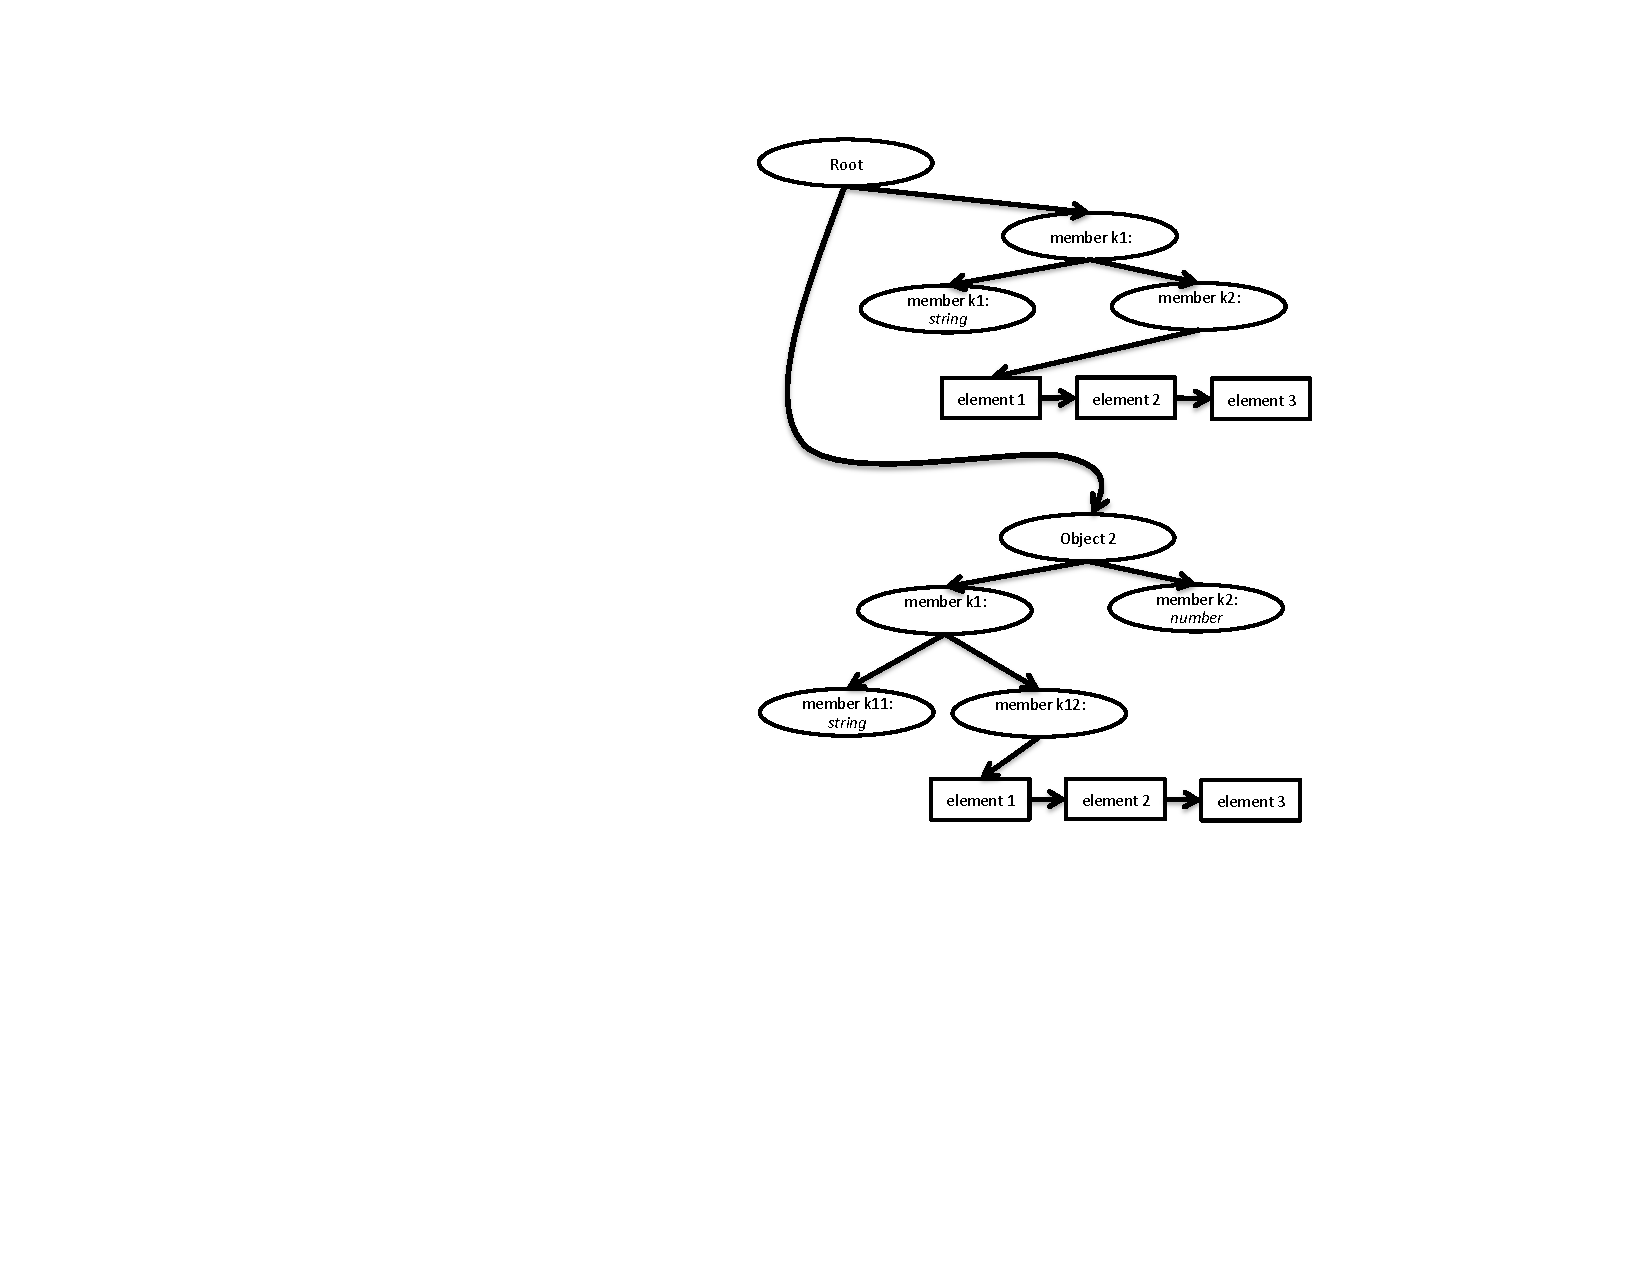
\includegraphics[height=2in]{json.pdf}
% \caption{A JSON document represented as a graph.  Note the nesting of JSON objects (key-value collections) in a tree shape of oval nodes, and lists as chains of rectangular nodes.}
% \label{fig:json}
% \end{minipage}
% \hspace{0.1\textwidth}
% \begin{minipage}{0.4\textwidth}
% 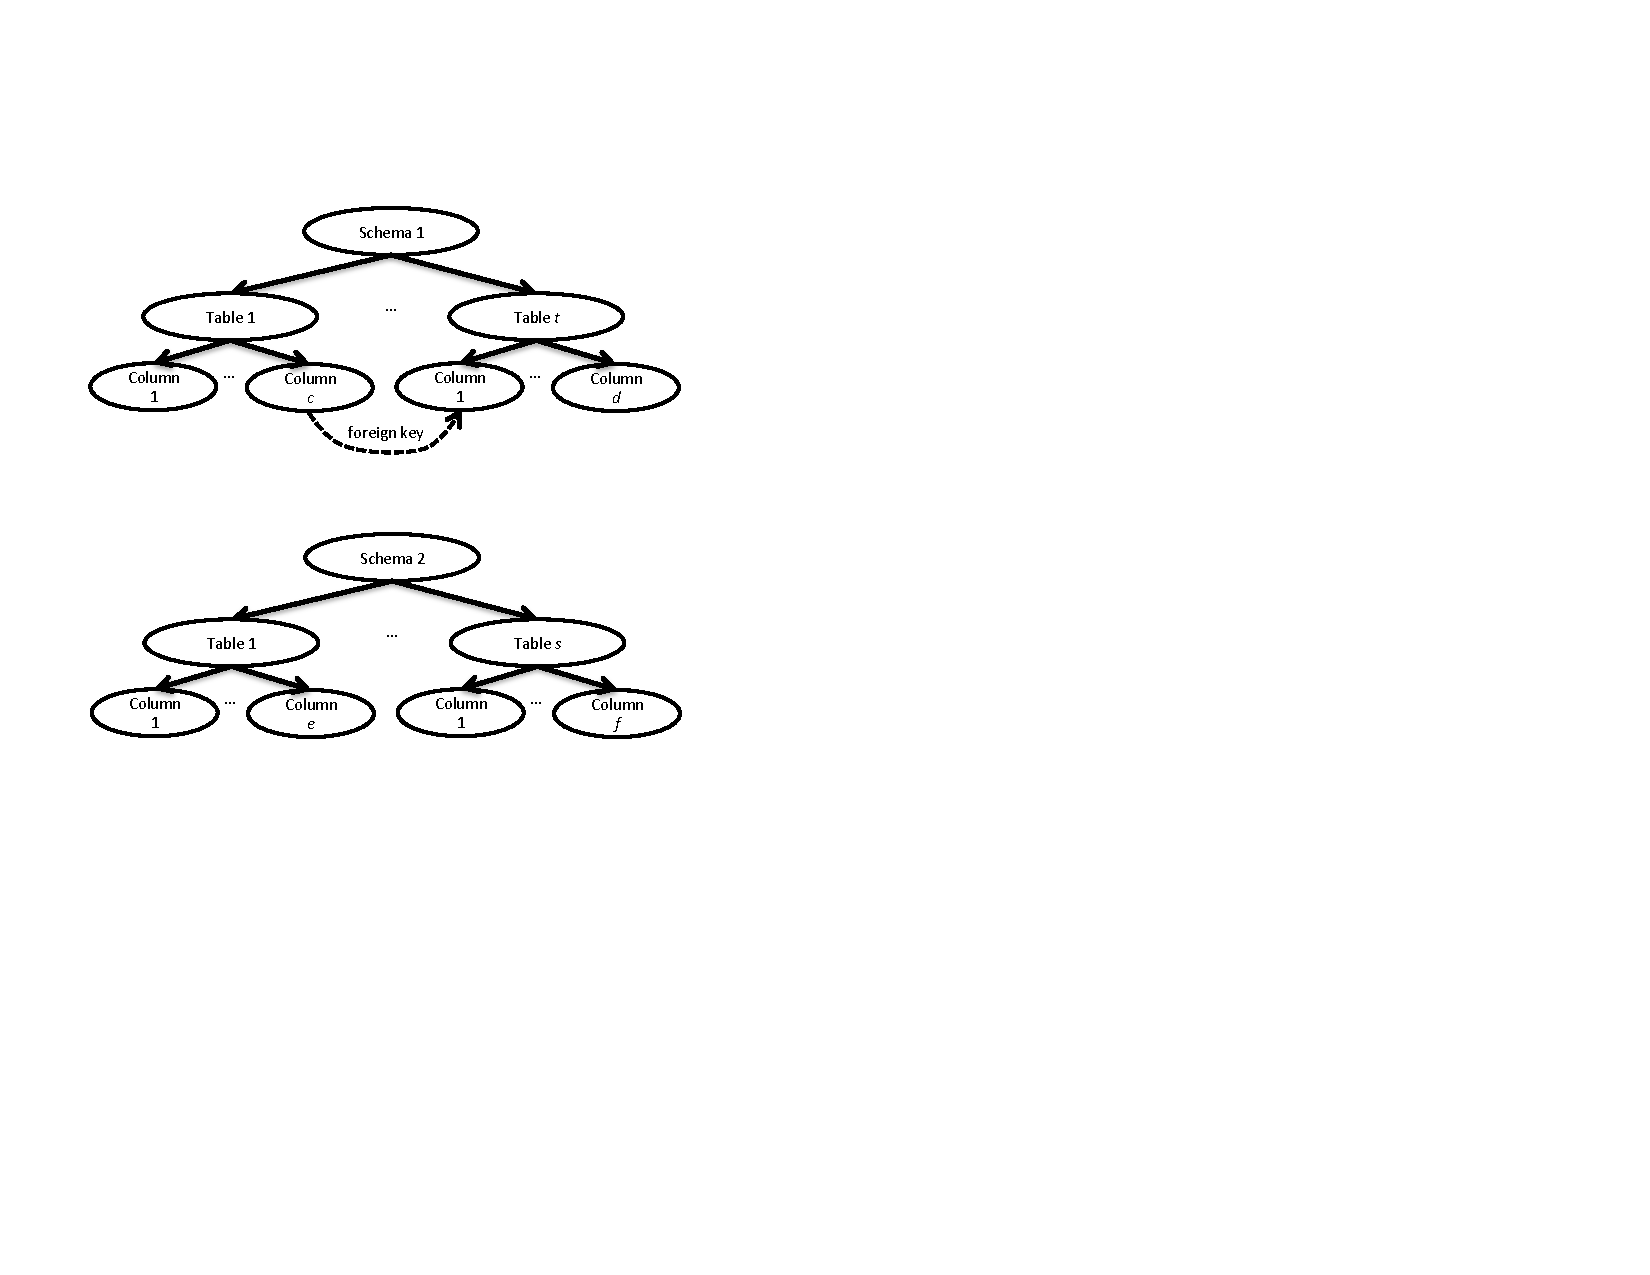
\includegraphics[height=2in]{relational.pdf}
% \caption{A relational database with two schemas, represented as a graph.  Note the fixed schemas$\rightarrow$tables$\rightarrow$columns structure, and
% the ad hoc foreign key references at the leaves.}
% \label{fig:relational}
% \end{minipage}
% \end{figure}

The basic structure of the \mantle model is defined by pairs of classes \texttt{$C$} and \texttt{$C$Version} (e.g. \node and \texttt{NodeVersion}, etc.)
These classes inherit from the \core model's \thing and \version classes respectively, imbuing a unique id as well as a \texttt{VersionHistoryDAG} with each instance of $C$.  
% In turn, all {\version}s in a subclass like
% \texttt{NodeVersion} are identified by a \texttt{TVID} (Version ID) that stores
% both the ID of the corresponding \thing , and another \texttt{VersionID}
% to distinguish the specific \version.  
% It is thus possible to determine {\thing}s
% from their {\version}s and vice versa.  
% \jmh{There is a 1-to-many constraint
% between {\thing}s and {\version}s.  Worth noting, and asserting somewhere in the
% code.} \vikram {We agreed that we didn't need actually add anything about this
% to the document, right?}

To provide customization, the \mantle metamodel supports
both ad hoc {\gtag} key-value pairs, and fixed {\structure}s containing a prescribed set of {\gtag}s. 
% {\version}s themselves are
% immutable, so this information has to be associated upon creation. 
{\version}s and {\gtag}s are immutable; adding a ``new'' tag to a \thing creates a fresh
\version. By contrast, {\structure}s have associated \texttt{StructureVersion}s to capture their evolution; {\version}s are (optionally) associated with a specific \texttt{StructureVersion}, not a \structure.
\jmh{I skipped over RichVersions for simplicity.}
  % {\tag}s refer to the {\version} that contains them; 
  %a \tag is uniquely identified by its \version and key.  
% , a new \version subclass (e.g. \texttt{NodeVersion}) must be generated to hold the new {\tag}s, and linked as a successor into
% the \texttt{VersionHistoryDAG} of the corresponding \thing\footnote{Logically,
% the new version would likely contain a copy of all the unmodified {\tag}s
% of the preceding version as well, though in an implementation this could be
% encoded more efficiently.}.  
% We also allow {\tag}s to be associated with {\thing}s, 
% enabling users to register immutable tags that apply to all versions of a \thing.  \jmh{Need to get 
% this into the code.}  
% Structured information is captured via a \structure, akin to a relational table schema or a C struct. (This class is a descendant of \thing, hence contains versions in the form of \texttt{StructureVersion}s.) {\structure}s provide a prescribed metadata format
% consisting of a set of key-type pairs; each \version that references a given \texttt{StructureVersion} 
% \emph{must} have {\gtag}s with the corresponding 
% keys and value types.

% Up to this point we have referred to types rather loosely.  Ground currently includes 
% a typical set of built-in atomic types common to most languages: booleans, characters, strings, and
% numerics.  For now most of these types are being taken from Scala; we will evaluate whether additional 
% atomic types (e.g. SQL's decimal type) need to be built in.  One important type that is specific to 
% Ground is the Uniform Resource Identifier, or \uri.  We will describe the use of {\uri}s in more detail in the next section.  As of now we have no plans for user-defined types in Ground, though we will revisit
% this decision as we progress.
% As noted above, basic {\version}s are simply unique identifiers.
% We define {\richversion}s, which can be augmented with {\gtag}s and \texttt{StructureVersion}s.  Our main user-facing modeling classes inherit from \richversion to support customization.  In general, the immutable aspects of \mantle model objects are captured in a \thing subclass
% (e.g. \node), and the mutable aspects in the corresponding \richversion subclass (e.g.
% \texttt{NodeVersion}).  


% These basic objects are quite simple, but they can be customized by attaching
% ad hoc \texttt{Attributes} to their versions: these are key/value pairs that can
% be attached to a specific \version. \jmh{Not clear from the Scala how you get attributes of a \thing!}
% Optionally, {\version}s can also have a \texttt{Structure} that they impose: a set of attributes
% that they must contain.
% This more complex
% metamodel will simply be a composition of the building blocks we highlighted.
% The \mantle serves as the basis for increasingly rich, use-case specific forms of metadata that can be structured on top of this intermediate
% metamodel, benefiting both from the versioning embedded in the \core, and
% the typed graphical structure of the \mantle.

The critical \mantle subclasses are \node and
\texttt{NodeVersion}, \edge and \texttt{EdgeVersion} and \graph and
\texttt{GraphVersion}, all defined in a straightforward manner.
% The \node, \edge and \graph classes contain no more information than the \thing superclass provides; similarly the 
% \texttt{NodeVersion} class contains no more than \version.
% %, albeit in a publicly visible interface.
% % However, both the
% % \texttt{NodeVersion} and \texttt{EdgeVersion} classes augment their \version
% % superclass with an optional reference to a \texttt{StructureVersion} (that we
% % will describe shortly) to represent a required structure for the version.
% By contrast, \texttt{EdgeVersion}s add two \texttt{NodeVersion} endpoints; \texttt{GraphVersion}s contain a set 
% of \texttt{EdgeVersion}s.  
% Like other properties of a \version, that set is immutable.  Hence a new 
% \texttt{GraphVersion} needs to be generated to capture the \graph being modified by insertion,
% deletion, or update of an existing \texttt{EdgeVersion}.

  % Working through the definitions of
% Figure~\ref{mantle} you can see straightforward definitions of \texttt{Set}s
% and \texttt{SetVersion}s, which inherit from \thing and \version.  The \graph
% class inherits from \texttt{Set} without modification; the
% \texttt{GraphVersion} class extends \texttt{SetVersion}.

  % \jmh{For symmetry, we should probably rename \version to Version, and \thing to something else like a Thing.} \jmh{We need a naming convention for these things to avoid the goo of discussing objects and versions in an ad hoc way.}


% In the \mantle metamodel, we have a number of objects that each extend the
% \texttt{VersionedItem}. For each of object (say) ``\texttt{Foo}'', there is a
% corresponding ``\texttt{FooVersion}''
% class.
% These classes extend the \version class and compose the \texttt{VersionHistoryDAG}
% for the objects that they represent.

% We also have collections of {\node}s and {\edge}s. In order to illustrate the
% design of these collections, let's consider the example of a \graph, which is
% represented simply by a set of {\edge}s. A \graph, just like all the other objects
% in the \mantle, is a \thing. 
% Versions are more complex for a collection type like {\graph} than for scalar types like \node or \edge.
% A \graph's version can change in two different ways. The first is simple: when you add or delete an \edge from the \graph, you implicitly create a new
% version of the \graph container. The
% second is if the {\edge}s themselves are modified---in particular, when the
% endpoints of the \edge change, even though the identity of the edge may not\footnote{As a motivating example, consider an ``ownership'' \edge that represents the current owner of a file.  This fact does not change identity, it just links to a different principal as the owner, allowing us to track the ownership of that file over time.}. This second case poses an interesting challenge
% in terms of correctly propagating versioning changes. In order to solve this
% problem, every \thing has the capability of being ``watched''. That is,
% every object has a list of subscribers to which it publishes updates.
% In Ground, a \graph
% watches every one of its {\edge}s, and if an \edge is modified, then the \graph
% will also create a new version of itself with this \edge.  \jmh{This feels imperative.  Instead, how about a declarative description of a constraint: the version of a Graph relates in some way to the most recent version of any Edge it contains.  You could probably leave out the description of how this is achieved
% entirely.} \vikram{Maybe I'm not understanding what you mean by declarative
% here, but if you read up until the sentence that ends with "the identity of the
% edge may not, I think it describes the ways in which the identity of a graph
% depends on its edges. Beyond that, if we want to leave out a description of how
% we're accomplishing this, then we can just cut out everything after that,
% right? Or is there something else missing?}

\paragraph{External Things and Schr\"{o}dinger Versioning}
Lastly, we need to represent items outside of Ground that should be tracked: canonical examples
include code in GitHub, or documentation in Google Docs. These objects are represented in Ground by \texttt{ExternalThing}s, with \texttt {ExternalVersion}s that contain a various tags: a \uri reference,  timestamp, optional \texttt{cachedValue}, and parameters for accessing the
reference (e.g., port, protocol, etc.)
% \texttt{ExternalThing}s have an \texttt{isUnchanging}
% flag, which, if enabled, is an indication that the external resource is expected to be
% immutable, and there should only be one \texttt{ExternalVersion} associated.
% Note that this is advisory; if the actual reference changes, Ground will not be aware. 
Ground cannot automatically observe an external item's changes. Hence
% (i.e., not \texttt{isUnchanging}), 
API access to the \texttt{URI}
of a \texttt{ExternalVersion} results in a new \texttt{ExternalVersion} being generated, containing an new
\texttt{VersionID}, an updated timestamp and possibly an updated cached value. \jmh{pullquote} We refer to this as a \emph{Schr\"{o}dinger} versioning scheme: each time we observe an ExternalThing it changes.

% In summary, the \mantle model provides a public, above-Ground interface for building application-specific 
% abstractions by customizing the optional and structured tags of nodes and edges, and laying them out in versioned graphs. 

\subsubsection{\Crust Metamodel: Provenance Graphs}

% \begin{figure}[ht]
% \begin{scriptsize}
% \begin{multicols}{2}
% % \lstinputlisting{scala/crust.scala.txt}
% \end{multicols}
% \end{scriptsize}
% \caption{\Crust metamodel in Scala.}
% \label{fig:crust}
% \end{figure}
The goal of the \crust model is to capture usage information composed from the nodes and edges modeled in the mantle.  
% This usage is captured by \emph{provenance graphs} in the form of
% \texttt{LineageEdge}s.  To facilitate data lineage, Common Ground depends on
% a notion of \texttt{Principals} and \texttt{Workflow}s that we define first.  
% ; we believe they are fundamental
% to any metadata system as parameters of provenance.

\texttt{Principal}s (a subclass of \thing) represent the actors that work with data:  users, groups, roles, etc. 
% \texttt{Principal}s are particularly important in data governance
% because they are central to both auditing and
% enforcement of policies like access control.
% Note that \texttt{Principal}s
% are {\node}s, and built while access rights and group membership can be represented as {\edge}s.
% {\structure}s would be particularly useful here because users would
% have some set of required information based on the identity \& authentication
% schemes being used. 
\texttt{Workflow}s (a subclass of {\graph}) represent specifications of code invocation.
\texttt{Principal}s and \texttt{Workflow}s
are the only ``semantic'' metadata objects prescribed by Common Ground; the rest of the metamodel is 
 structural and generic.
Any Data Governance effort requires both of these classes: as examples, they are key to use cases involving
in-line enforcement, off-line auditing and reproducibility.

% The second common semantic concept is \emph{workflow specification}.
% This sort of metadata is very important to critical use cases like reproducibility and auditing.
% Workflows are representable in terms of the graph
% structure of the \mantle model, but we chose to make them
% first-class citizens in the \crust of the Ground metamodel. These
% This is critical to use cases like reproducibility and auditing.

% \texttt{Workflow}s
% can capture a sequence of \textit{ad hoc}, exploratory actions or a
% pre-defined sequence of actions. 

In Ground, lineage
is captured as a relationship between two {\version}s (of two possibly different subclasses), the second of which is derived from the
first. This relationship is due to some process, either computational
(workflows) or manual (via some principal). Basic \texttt{EdgeVersion}s as described
in the \mantle cannot reference other {EdgeVersion}s.  
So we introduce \texttt{LineageEdge}s, which contain 
optional references to \texttt{Workflow} and \texttt{Principal} nodes. As is well known in the data provenance literature~\cite{cheney2009provenance}, these lineage edges may be better computed on the fly by analyzing 
code; \emph{ephemeral} \texttt{LineageEdges} can be used to maintain the Ground lineage API without committing the (redundantly computed) \texttt{LineageEdges} to immutable storage.

\subsubsection{\groundwire: User-Defined Models}
The three layers of the Ground metamodel are intended to support a wide range of usage.
However, we expect users of the Ground service to interact with it via a language-agnostic API called \groundwire.  Users can define their own
customization of the Ground metamodel by declaring custom {\structure}s and {\gtag}s.  
These can be packaged into libraries for common cases (e.g. a library for representing
relational database catalogs, or a library for representing JSON documents).  These libraries can 
be independent of each other, but based in the unified Ground model.  

% The API for \groundwire is the subject of a separate document.

%%%%%%%%%%%

\subsection{Key Services}
Ground's functionality is backed by five key subservices.  For agility, we are starting the project using existing open source subservices wherever possible.  We anticipate that some of these will not work out, and that new research opportunities will emerge at the systems level.

\smallitem{Versioned Metadata Storage}.  Ground must be able to efficiently store and retrieve metadata with the full richness of the Common Ground metamodel, including flexible version management, data modeling and lineage storage.  Ground also needs to reference external data, which can come in arbitrary form, with a wide variety of APIs, and handle Schr\"{o}dinger versioning.  The Common Ground metamodel imposes a unique set of requirements that goes beyond the built-in features of typical storage systems. In Section~\ref{sec:perf} we examine a range of candidate open-source systems; as noted there we believe this is an area for significant database research.

% Note that Ground is not intended as the primary interface for accessing the data that is referenced by metadata; Ground is expected to \emph{describe} external data and track it, not serve it.  Hence Ground's most basic requirement for external data is to know how to store a unique ID for each item it tracks, and return that ID to applications that request it.  In an ideal setting, each external data item is versioned, hence each version has a unique ID.  However if the external item is mutable and not versioned, Ground generates \emph{Schr\"{o}dinger versions} lazily: each time we observe an object we assume it changes, and assign it a new version (and version ID).  
% This is discussed in more detail in the Common Ground design~\cite{commonground}.

% \textbf{MVP:} We are currently mapping our metadata model onto a traditional PostgreSQL relational database for storage.  Graphs can be represented as relations, so we manage versions, lineage and data modeling graphs at application level above the relational model.  PostgreSQL is a fairly mature system but is not designed to meet our requirements for latency, scalability and availability. In fact we do not expect any relational solution to work well for our needs over time, as relational databases are not designed for any of the three key individual aspects of the metamodel: versioned data, polyglot data models, or rich lineage.  Unfortunately, we do not expect that solutions in the NoSQL or graph database world will fare well either, though this requires research to validate. Therefore a critical thrust of the Ground research agenda is to understand the weaknesses of existing database systems when faced with these requirements, and design a new database system that is well-suited to emerging metadata workloads. \jmh{Need to call out research hypotheses more clearly.}


\smallitem{Search, Update, Analyze}.  As noted above, Ground is intended to be permissive in the kind of metadata it stores.  First, it needs to support a least-common denominator of unstructured tags, and provide efficient search over those tags.  To this end it needs search-style indexing.
%; we plan to integrate Solr~\cite{solr} and ElasticSearch~\cite{elasticsearch}.  
Second, Ground needs to support efficient interactive behavior for applications that are inserting, updating and fetching metadata---capturing changes with versioning. Third, intelligent applications like those in Section~\ref{sec:scenarios} will run significant analytical workloads over metadata---especially usage metadata which could be quite large.  Finally, it seems natural that some workloads will need to combine these three classes of queries, perhaps via a federated query layer above them.  As we explore in Section~\ref{sec:perf}, various open-source solutions can address these workloads at some level, but there is significant opportunity for research here.

% \textbf{MVP:} Initially we are not supporting search or analytic APIs; these will be added as the system evolves.  For interactive query, we can only do as well as our prototype relational metadata store.  For search, we expect that existing solutions like Solr will be sufficient for the foreseeable future; we do not expect metadata tagging and querying to exceed volumes that Solr sees in free-text indexing. For analytics, we intend to leverage Spark and GraphX as we have significant expertise in house.  However, the nature of the analytics to be done here represents a major research opportunity: what might be the value of metadata in a Big Data context, and how could that value be extracted by analytics?  Could a \emph{self-aware} Big Data ecosystem improve itself, or provide valuable insight about its usage to applications and users?  \jmh{Again, call out research.}  Finally, the requirements for a federated query layer and its design are a topic for investigation after we acquire a corpus of metadata and workloads.

\smallitem{Ingestion: Insertion, Queues and Crawlers}.  Metadata may arrive to be stored in Ground interactively or in batches; it may be pushed in or need to be actively crawled.  
% Interactive insertion of metadata needs to be supported efficiently by the metadata storage component; batch insertion should make use of queueing services to handle bulk delivery and bursty arrivals.  
% Passive insertion needs to be handled via a data crawler that can register metadata from external services with Ground, and see if 
As references to data arrive in Ground, the Belowground ingestion API publishes notifications to Aboveground services like file parsers and feature extractors, which can augment the ``plumbing'' of metadata arrival with custom intelligence in generating metadata.  Subscribing applications Aboveground can fetch the referenced data as it arrives (or later), and enrich the inbound metadata with custom features.  We are currently working with existing open-source solutions for the Underground plumbing: Gobblin for crawling metadata~\cite{gobblin} and Kafka~\cite{kafka} for queueing and pib-sub to the Aboveground API. The Aboveground metadata extraction is of course a large research opportunity spanning database and AI research of various kinds; we hope that commodity APIs for scalable, continuous crawling and ingest of Big Data will drive more work in this area. Similarly, this is a rich area for industrial collaboration: the vendor-neutral aspect of Ground's plumbing should foster a healthy ecosystem for competition at higher levels.

% \textbf{MVP:}  Currently we are handling ingest solely via simple push insertion APIs that call into our metadata store via SQL.  However we envision integrating open-source solutions like Kafka for queuing, and Gobblin for crawling and data ingest from remote sources.  We are also eager to explore APIs to plug in third-party solutions for  extracting metadata from crawled data; two examples we are OpenCalais (a free automated service for entity extraction) and Trifacta (a commercial, semi-automatic solution for data transformation).  We also recognize that there are boundless R\&D opportunities here, some of which could be part of Ground, many of which should exist as standalone solutions above Ground.  \jmh{another research opening, though more about opportunities above ground.}  We look forward to integration with other research and non-research colleagues here.

\smallitem{Identity and Authorization Integration}.  Identity management and authorization are a required aspect of the Ground service.  The primary reason not to ``bake this in'' to Ground is administrative: most organizations already have an authorization service that the metadata service must use.  More importantly, authorization is a semantic notion with wide flexibility: the policies of a federal defense agency are likely to be wildly different in nature from those of a corporate marketing department, which in turn differs from a consortium of scientists interested in reproducibility.  The flexible design of Ground's metamodel should support a wide variety of authorization metadata (ownership, auditing, content labeling etc.) and design policy over that metadata.  An open design question is whether Ground needs to \emph{enforce} policy, or merely store it and notify Aboveground applications.  As another open question, note the subtle connections between metadata versions and policy versions, particularly when the authorization policies of a past time are considered unsafe later---what should be done retroactively? This is a case where good people may disagree about the virtues of immutability and reproducibility. More research is required here.

% \textbf{MVP:}  The current MVP has no support for identity management and authorization.  However our initial use case has us tracking UC Berkeley student IDs, Github identities, UNIX uids from instructional computing, and associations between the three; visibility of things like grading scripts and their outputs will depend on policies regarding these identities.  In the short term we expect to integrate with Google oAuth services as exposed at UC Berkeley next, and to explore the way that policy is specified and possibly enforced in our prototpype environment.  Our longterm roadmap here remains open; we expect a need to collaborate closely with partners in application domains to get further requirements.  \jmh{Possible tie to Raluca's work here, at minimum as an example of a non-standard approach to these issues.}

\smallitem{Scheduling, Workflow, Reproducibility}. We are committed to ensuring that Ground is flexible enough to capture the specification of workflows at many granularities of detail: from black-box executables to workflow graphs to source code.  However, we do not expect Ground to be a universal provider of workflow execution or scheduling; instead we hope to integrate with a variety of schedulers and execution frameworks including on-premises and cloud-hosted approaches. This is currently under design, but the ability to work with multiple schedulers has become fairly common in the open source Big Data stack, so we have examples to follow.

% \textbf{MVP:} We plan to begin by utilizing the scheduling and execution services provided by the Gobblin project, which supports a variety of schedulers including Quartz, Azkaban and Oozie, and execution frameworks including Yarn and Helix.  We plan to look into support for VMs and containers as well.  \jmh{Certainly could paint a research picture here, closer to the Bloom-meets-Kubernetes agenda: how will data-centric workflows be programmed in the future, especially as we look at containers, elastic services, etc?}  maybe also a connection to the Shenker/Jackson work on Declarative Datacenters?

\smallitembot
% \begin{figure*}[th]
% \center
% 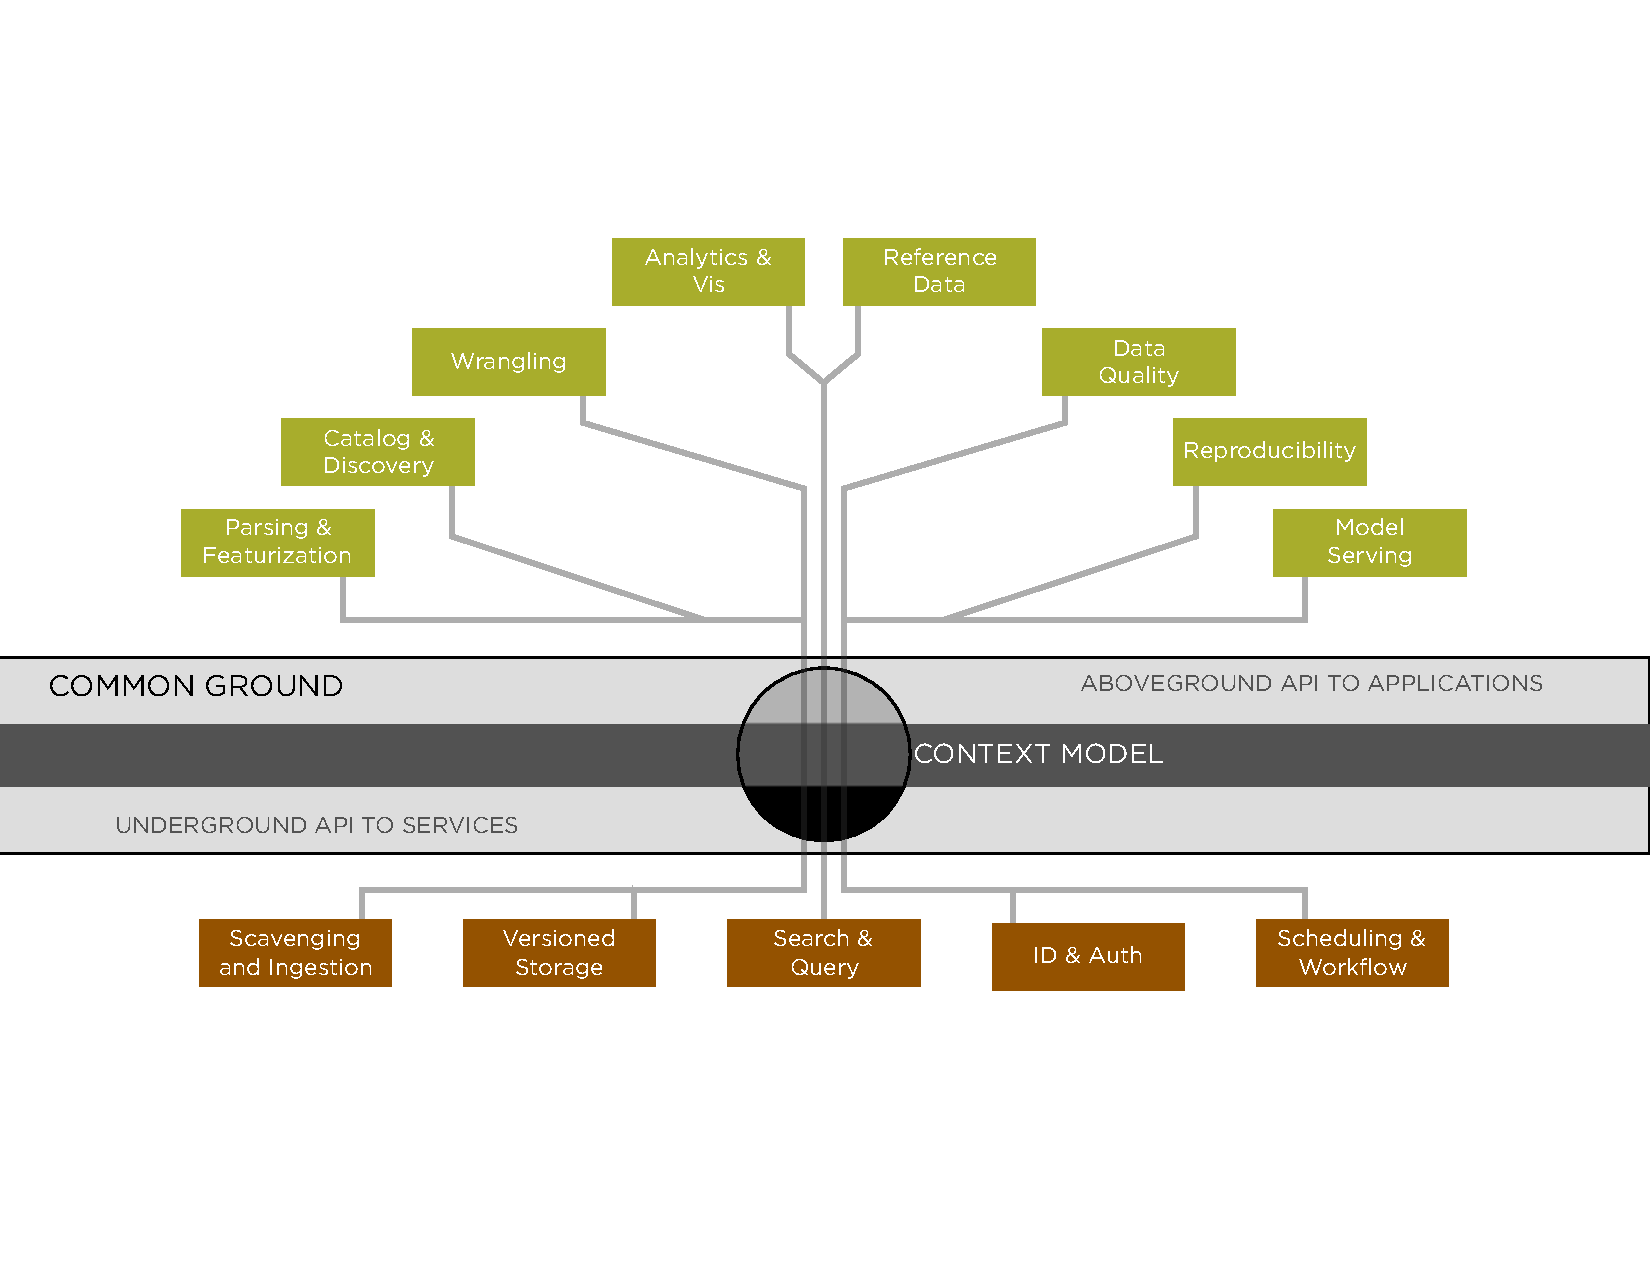
\includegraphics[width=0.7\linewidth]{groundarch.pdf}
% \end{figure*}

% \subsection{Common Ground: A Metamodel}
% \label{sec:metamodel}
% \subsection{Underground Services}

\section{Storage: A Prototype Evaluation}
\label{sec:storage}

An initial focus area in our prototype of Ground has been evaluating the current state of play in storage engines. We layered our data model on top of a number of existing open-source storage systems, namely, Postgres, Apache Cassandra, TitanDB, and Neo4j. We then evaluated the data model in a number of different scenarios. 
\vikram{These subsections need to be renamed. These are just placeholders for the time being.}
\subsection{Evaluation Scenarios}

\smallitem{Relational Metadata} One very common type of metadata is the relational schemas that are stored in the Hive Metastore. As a part of our prototype, we have built a connector that allows Ground to serve as a drop-in replacement for the existing Hive Metastore. One major benefit of using Ground as Hive's relational catalog is that schema versioning naturally falls out of this set up. 

\smallitem{Code Versioning} Another key kind of metadata is code versions. An integral part of tracking data usage effectively is understanding which code versions were used to transform or wrangle data. To that end, we have ingested version history graphs from git repositories into Ground. Combined with versioned 

\smallitem{Log Storage} The current state of log analysis tools often revolves around anomaly detection and error correction. However, logs often contain interesting usage data that is currently not being analyzed or leveraged in any way. As a first step, we took an Apache web server log and extracted user session metadata. We used this session data to detect potentially interesting trends, which we will discuss in more detail in the next section.

\smallitem{HDFS Metadata} Lastly, we have built a pipeline using Gobblin and Apache Kafka that extracts file system metadata from HDFS and writes to a Kafka topic, which is then ingested into Ground. This pipeline notifies us of any new files that are added to HDFS. In addition, we are planning on adding hooks which allow Ground to call out to other services (e.g., a parser or featurizer that will extract additional metadata) that might be interested in new files. 

\subsection{Evaluation Functionality}

Functionality:
\begin{itemize}
\item transitive closure
\item point lookup
\item sessionization and trends?
\end{itemize}

Performance/Scale.

\section{Discussion}
\label{sec:discussion}
\jmh{This may evolve into Research Opportunities or Future Work, but this is a placeholder for things that were postponed in earlier text}

\jmh{Backref to Scalability discussion above, and the question ``are logs data or metadata''?}
Functionality: well, we've started building out a few things and they went well.  Apiary and Grit.

Performance: Here we ran into some bottlenecks with the widely-used storage systems in the field.  This merits more attention.

\subsection{Initial Results}
\label{sec:perf}

\section{Challenges for the community}
\label{sec:challenges}
\jmh{May not be room for this. Instead find a way to call out the challenges in the body as they occur, with clear formatting.}

\section{Related Work}
\label{sec:relwork}
\jmh{I think we can give a ``sketch'' for the submission version.}
Related work comes in a variety of categories, and we give a sketch here; representative citations for each of these categories will be included in the final paper. 
Historical Master Data Management and ETL designs are ill-suited to modern data context as they were built for schema-on-design data warehousing.  But they provide good examples of data lineage and governance features to enable in a more agile world. Recently, two ``context service''-like systems are under development at Google (Goods) and IBM (labbook), illustrating the potential in this space. \jmh{Need to read papers and call out differentiators and lessons. Goods may be like WhereHows---a specific use case. LabBook might be more close to us.}  
In the Big Data world, there are two emerging metadata service options that are targeting general-purpose use: Cloudera Navigator and Apache Atlas led by Hortonworks and their customers. Both of these are built on a flexible graph metamodel that inspired the Common Ground \mantle metamodel; neither provides the \core versioning we propose, and neither is perceived as a vendor-neutral option by customers.  These solutions are also exploring ``underground'' alternatives for storage and querying, and there is innovation to be shared among them. Custom metadata stores have been open-sourced by LinkedIn (WhereHows) and FINRA (Herd); both of these are ``opinionated'' rather than general-purpose: specific to use cases in their organizations. They provide a good challenge for Ground, as examples of use cases to be supported. Finally, there is a wide variety of work in both research and industry on isolated, full-stack (smokestack) applications for particular kinds of context usage, including Big Data catalog applications (Alation, Tamr, Waterline), analytic lineage systems (ReproZip, Burrito), information extraction systems (DeepDive, OpenCalais, etc.) and so on. Our hope is for Ground to provide a widely adopted, interoperable subsystem for these applications, freeing them to focus on their own key technical differentiators in adding application-specific intelligence and user experiences.  Finally, there is a host of research on graph queries/DBs, and a much smaller body of work on immutable databases (Postgres, Datomic, Pachyderm.io, Noms); it is quite possible that those solutions could evolve to serve the needs of a context service like Ground.
\section{Conclusion}
\label{sec:conclusion}
\jmh{Fire up the reader ... leave on a note of potential impact and open research opportunity. Maybe two big buckets of future work Belowground and Aboveground if we skip ``Challenges''. In essence those two buckets cover most of database research today!  So this is a playground and dogfood all at once, to mix metaphors badly.}

\begin{figure*}[th]
\centering
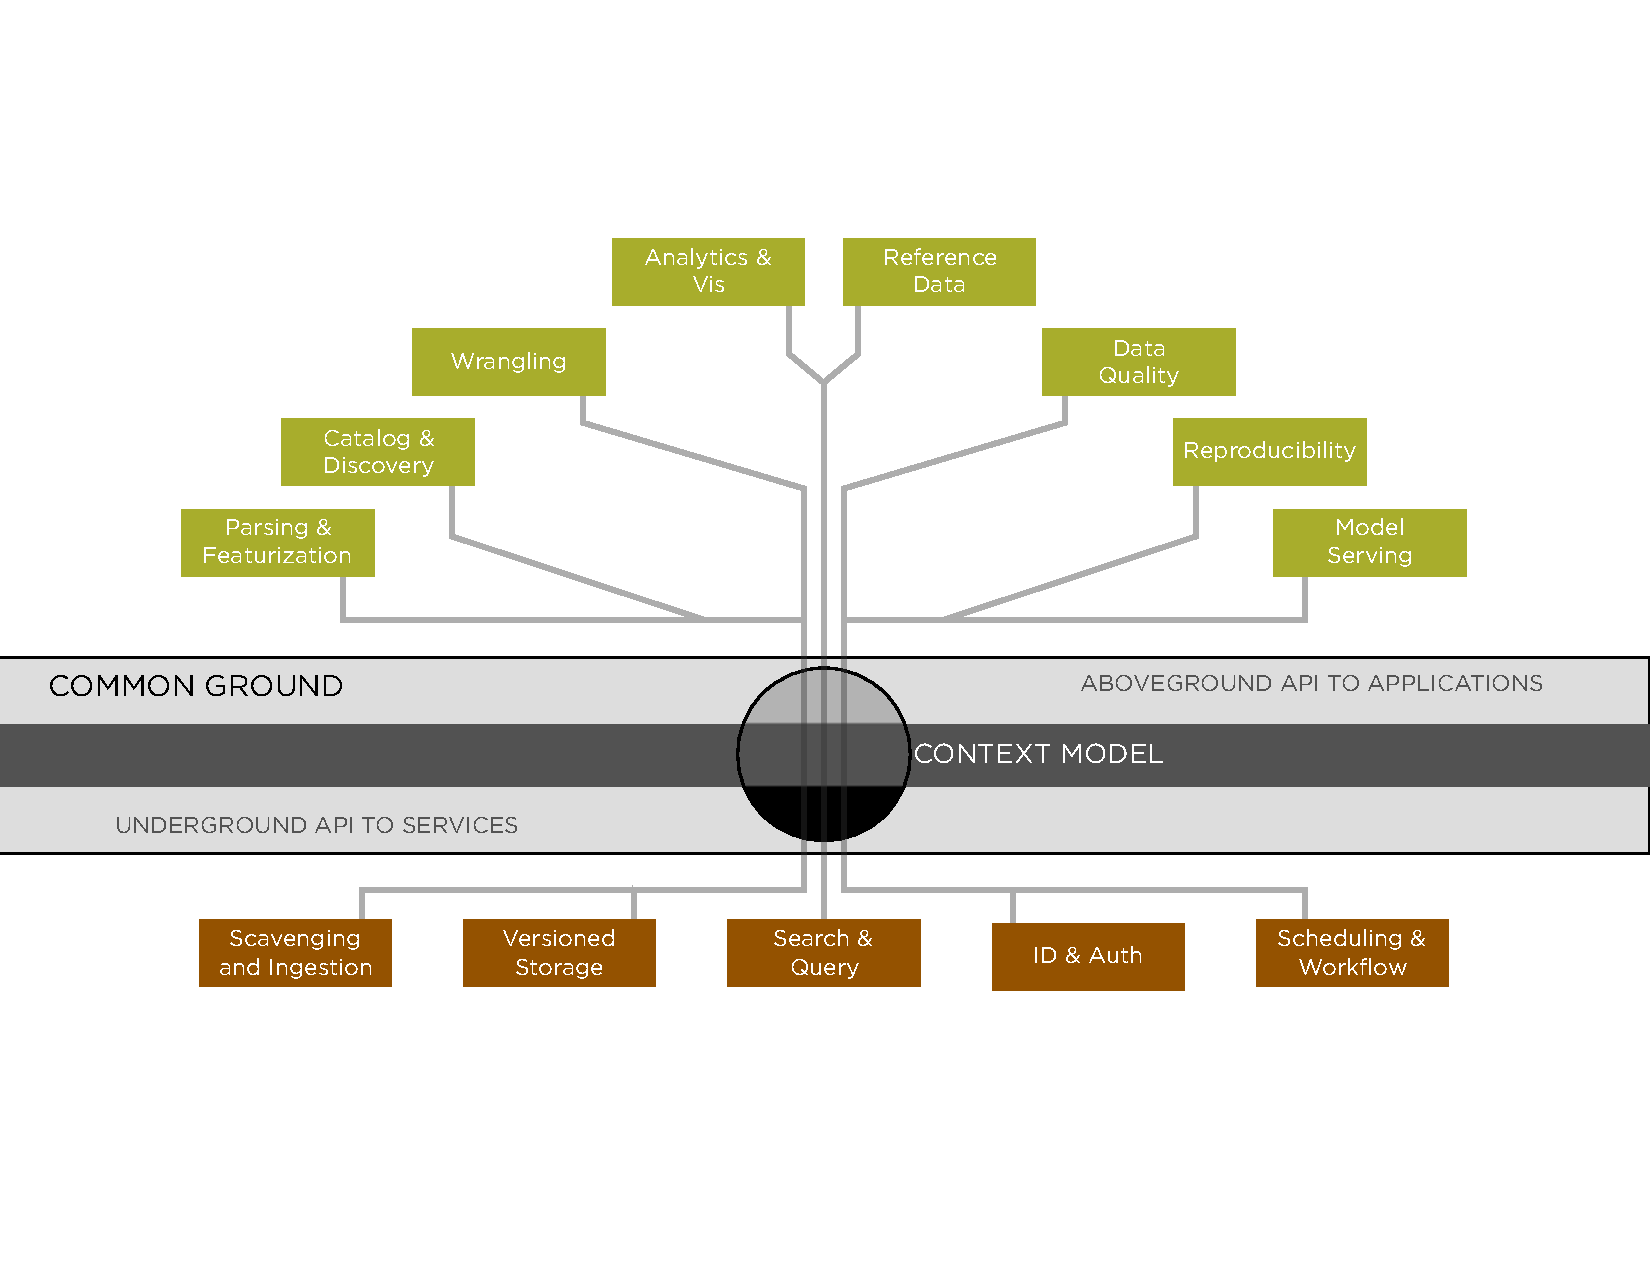
\includegraphics[width=0.75\linewidth]{groundarch.pdf}
\caption{A sketch of the Ground architecture.}
\label{fig:arch}
\end{figure*}

\begin{figure}[th]
\centering
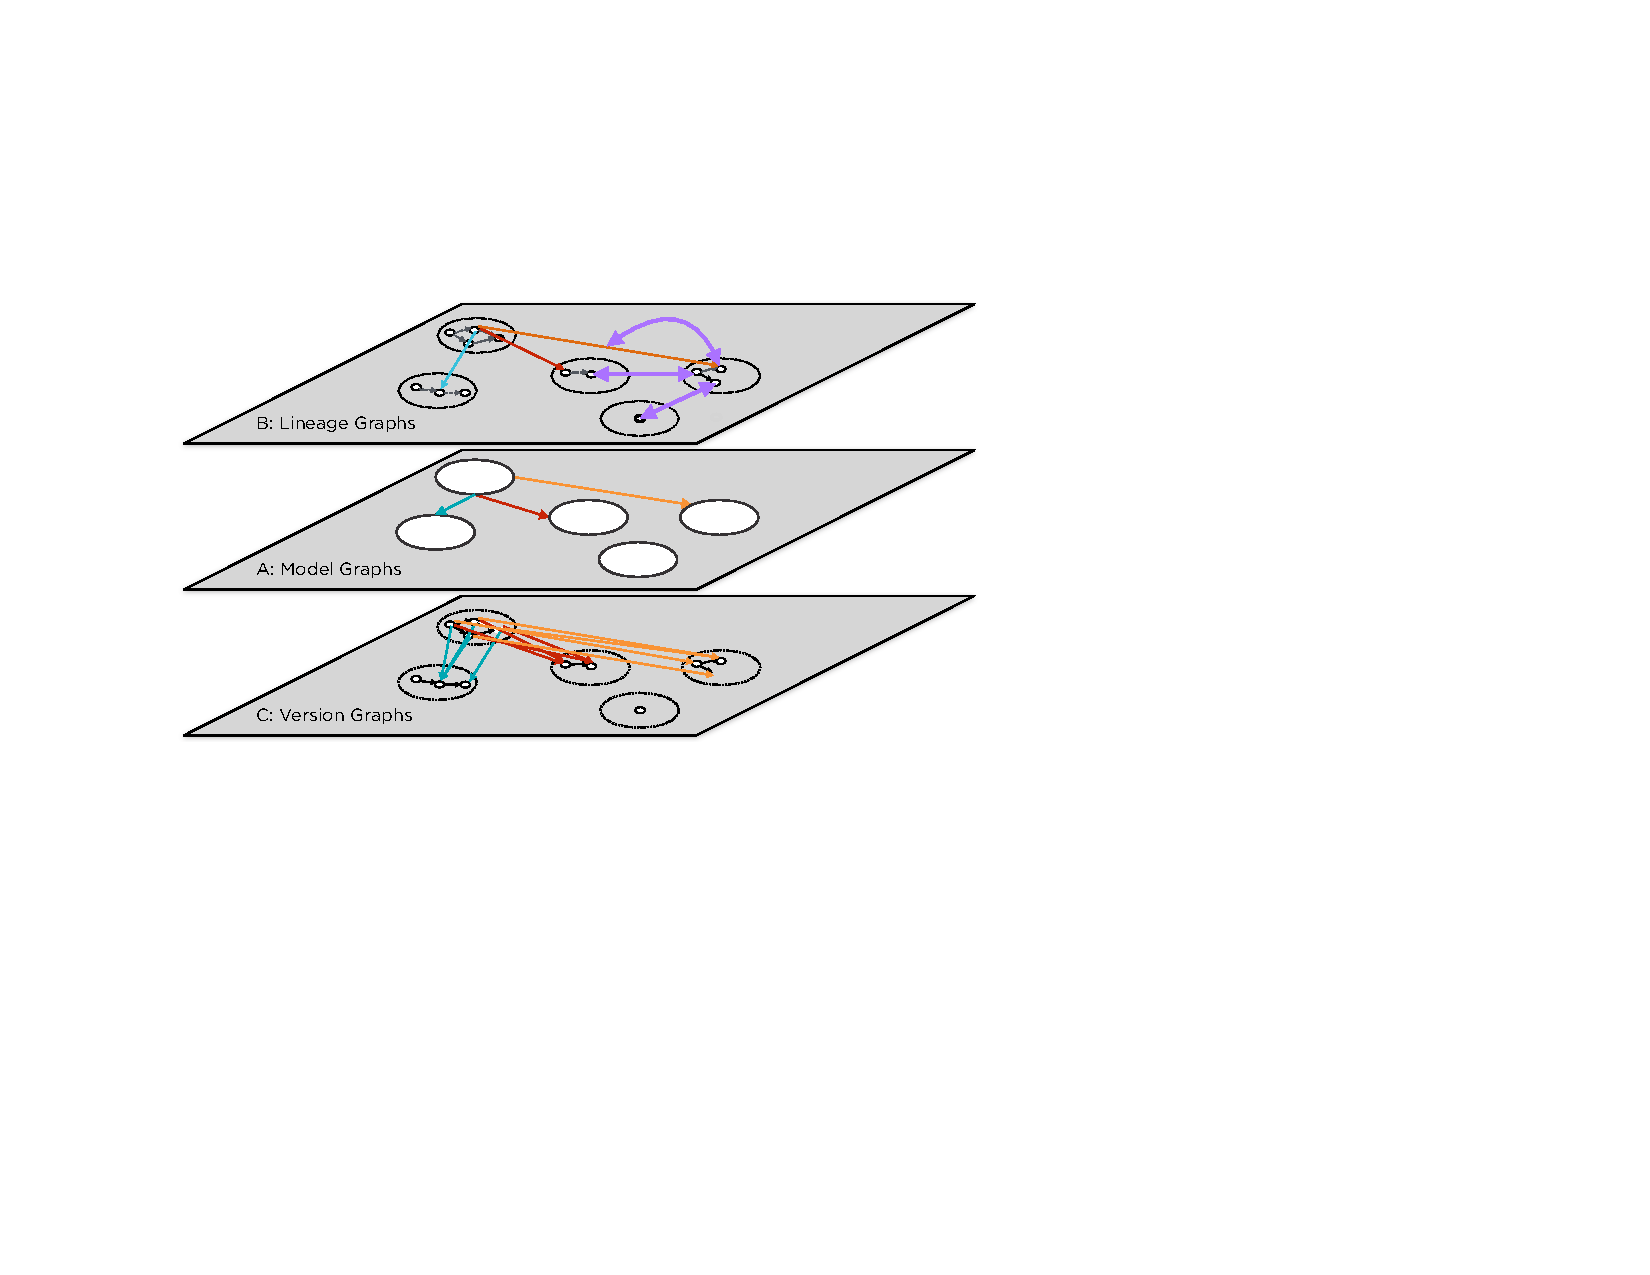
\includegraphics[width=0.75\linewidth]{layers.pdf}
\caption{The \vml model.  The central layer shows {\node}s (circles) and {\edge}s.  
Below are corresponding \texttt{NodeVersion}s (small dots) connected by \texttt{EdgeVersion}s.  
Above is an example of lineage (dark edges) among selected versions.
% For simplicity, the figure omits \texttt{VersionSuccessor} relationships between different \texttt{LineageEdgeVersion}s at the top, and between \
% \texttt{EdgeVersion}s in the bottom layer.
}
\label{fig:layers}
\end{figure}


\bibliography{ground}
\end{document}
